\documentclass{article}

\usepackage{latexsym}
\usepackage{fancyhdr}
\usepackage{algorithm}
\usepackage[noend]{algpseudocode}
\usepackage{amsmath}
\usepackage{amsthm}
\usepackage{amssymb}
\usepackage{mathtools}
\usepackage{amsthm}
\usepackage{bbm}
\usepackage{hyperref}
\usepackage{listings}
\usepackage{scrextend}
\usepackage{dirtytalk}
\usepackage{titlesec}
% \usepackage[demo]{graphicx}
\usepackage{caption}
\usepackage{subcaption}
\usepackage{pdfpages}
\usepackage[shortlabels]{enumitem}
\usepackage[margin=1.2in]{geometry}
\lhead{Charles Pehlivanian}
\rhead{Consecutive Partitions For Power Score Functions}
\cfoot{\thepage}
\pagestyle{fancy}


\setcounter{secnumdepth}{4}


\hypersetup{colorlinks=true, urlcolor=blue}

\newcommand{\ignore}[1]{}

\newtheorem{thm}{Theorem}
\newtheorem{definition}{Definition}
\newtheorem{lemma}{Lemma}
\newtheorem{sublemma}{Lemma}[lemma]
\newtheorem{corollary}{Corollary}
\newtheorem{prop}{Proposition}

\newtheoremstyle{case}{}{}{}{}{}{:}{ }{}
\theoremstyle{case}
\newtheorem{case}{Case}

\DeclareMathOperator*{\argmax}{argmax} % thin space, limits underneath in displays
\DeclareMathOperator*{\argmin}{argmin} % thin space, limits underneath in displays
\newcommand{\stirlingii}{\genfrac{\{}{\}}{0pt}{}}

\newenvironment{example}[1]{\par\noindent\underline{Example:}\space#1}{}

\newenvironment{claim}[1]{\par\noindent\underline{Claim:}\space#1}{}
\newenvironment{claimproof}[1]{\par\noindent\underline{Proof:}\space#1}{\hfill $\blacksquare$}

\makeatletter
\def\BState{\State\hskip-\ALG@thistlm}
\makeatother

\begin{document}
\sloppy

\begin{abstract} 
	[REVISE-OUTDATED] We consider....\end{abstract}

\section{Preliminaries}
Let $n \in \mathbb{N}$ be positive and set $\mathcal{V} = \{1, \dots, n\}$. Let $X = \left\lbrace x_1, \dots, x_n\right\rbrace$, $Y = \left\lbrace y_1, \dots, y_n\right\rbrace$ be finite real sequences with $y_i > 0$, for all $i$. 
It is assumed that $X$, $Y$ are orderd to satisfy $\frac{x_1}{y_1} \leq \frac{x_2}{y_2} \leq \dots \leq \frac{x_n}{y_n}$. In many applications, the tuple $(x_i, y_i)$ corresponds to occurence and baseline attributes for $i$, possibly associated with a spatial location. Denote by $\mathcal{D} = \mathcal{D}_{X,Y}$ the set of tuples $\left\lbrace \left( x_i, y_i\right) \right\rbrace$ associated with $X$, $Y$. $\mathcal{D}$ is assumed to have an order induced by a priority function on the sequences $X$, $Y$. A partition $\mathcal{P} = \left\lbrace S_1, \dots, S_t\right\rbrace$ of size $t$ of $\mathcal{V}$ can be identified with a pointset in $\mathbf{R}^2$ by associating $S \subseteq \mathcal{V}$ with the point $(\sum_{i \in S}x_i, \sum_{i \in S}y_i)$, called the $\textit{partition point}$ of $S$. Set $p_{\emptyset} = (0,0)$. In this way the sequences $X$, $Y$ induce an embedding of $\mathcal{P}$ into $\mathbf{R}^2$. The notion of score function comes from the spatial scan statistics literature.

\begin{definition}
A score function is a continuous $f(x, y)\colon \mathbb{R} \times \mathbb{R}^{+} \to \mathbb{R}$, nondecreasing in $x$, with continuous extension to the origin in any wedge $\mathcal{W}\left(\mu_1,\mu_2\right) = \left\lbrace (x,y) : y > 0, \mu_1 \leq \frac{x}{y} \leq \mu_2 \right\rbrace$, for $-\infty < \mu_1 \leq \mu_2 < \infty$, with the extension satisfying $f(0,0) = 0$. If $f$ is of the form $f(x,y) = x^\alpha y^{-\beta}$ for some $\alpha, \beta > 0$, then $f$ is a rational score function. 
\end{definition}

The regularity condition on $\mathcal{W}$ in wedges simply guarantees a continuous extension to the origin on any positive cone in $\mathbf{R}^+$, for rational score functions the constraint corresponds to the constraint $\alpha > \beta$. We do not assume smoothness beyond continuity, nor (quasi)convexity, etc., unless explicitly stated. The function $f$ induces a real-valued set function on $2^{\mathcal{V}}$ by defining $F(S) = f(\sum_{i \in S}x_i, \sum_{i \in S}y_i)$.  

For a given $f$, We are interested in maximal partitions for $F$, i.e., solutions to the program
\begin{align} \label{SetFMax}
\mathcal{P}^{*} = \argmax_{\substack{\mathcal{P} = \left\lbrace S_1 \dots, S_t\right\rbrace}} {\sum\limits_{j=1}^{t}F\left(S_j\right)} = \argmax_{\substack{\mathcal{P} = \left\lbrace S_1, \dots, S_t\right\rbrace}} {\sum\limits_{j=1}^{t}f( \sum_{i \in S_j}x_i, \sum_{i \in S_j}y_i)}
\end{align}
which for a rational score function is simply
\begin{align} \label{ScoreMax}
\mathcal{P}^{*} = \argmax_{\substack{\mathcal{P} = \left\lbrace \pi_1 \dots, \pi_T\right\rbrace}}\sum_{j=1}^{t}\frac{(\sum_{i \in P_j}x_i)^\alpha}{(\sum_{i \in P_j}y_i)^\beta}
\end{align}

\begin{definition}
A consecutive subset of $\mathcal{V}$ is a subset of the form $\left\lbrace j, j+1, \dots, k \right\rbrace$ for some $1 \leq j \leq k \leq n$. A consecutive partition $\mathcal{P} = \left\lbrace S_1, \dots, S_t\right\rbrace$ is a partition of $\mathcal{V}$ such that each $S_i$ is a consecutive subset. 
\end{definition}
Letting $\mathcal{P}_{c}$ be the set of consecutive partitions of $\mathcal{V}$, it is easy to see that  $| \mathcal{P}_c | = \frac{n(n+1)}{2} + 1$.
\begin{definition}
The score function $F$ satisfies the Consecutive Partitions Property (CPP) if the solution
\[
\mathcal{P}^* = \argmax_{\substack{\mathcal{P} \\ \vert \mathcal{P}\vert = t}} {\sum\limits_{j=1}^{T}F( \sum_{i \in P_j}x_i, \sum_{i \in P_j}y_i)}
\]
is a consecutive partition, for all $X, Y$. $F$ satisfies the Weak Consecutive Partitions Property (WCPP) if the solution
\[
\mathcal{P}^* = \argmax_{\substack{\mathcal{P} \\ \vert \mathcal{P}\vert \leq t}} {\sum\limits_{j=1}^{T}F( \sum_{i \in P_j}x_i, \sum_{i \in P_j}y_i)}
\]
is a consecutive partition, for any $X, Y$. $F$ satisfies CPP$(\mathbf{R}^+)$, WCPP$(\mathbf{R}^+)$ if it satisfies CPP, WCPP, respectively, for $X \subseteq \mathbf{R}^+$, $Y$.
\end{definition}

The following was shown in $\cite{PN}$

\begin{thm} \label{thm1}
Let $f(x,y) = x^{\alpha}y^{-\beta}$ be a rational score function with $\alpha > \beta > 0$. Then $f$ satisfies CPP if and only if $\alpha - \beta = 1$ and $\alpha$ is even. $f$ satisfies WCPP if and only if $\alpha - \beta \geq 1$ and $\alpha$ is even. 
\end{thm}

\subsection{Equivalence results for $X \subseteq \mathbf{R}^+$}
Formulations of equivalence results for the Theorems above are not immediately obvious as there are many extensions of the set function $F\colon 2^{\mathcal{V}} \to \mathbf{R}$ to the polytope $\mathcal{C}$. $\mathcal{C}$ is defined in terms of the give sequences $X$, $Y$ on a subset of $\mathcal{C}$ through the association $S \in 2^{\mathcal{V}}$ with $p_S \in \mathbf{R}^2$. Nonetheless, we may look for the existence of a suitable (convex, possibly subadditive) extension $f\colon \mathcal{C} \to \mathbf{R}$ in the context of a relaxation of the optimization in $\ref{eq1}$. Although our optimization is over partitions rather than subsets of $\mathcal{V}$, it is clear from the previous section that optimization over subsets is the basis of an iterative algorithmic approach (see below). We therefore start there. The standard approach for minimization of a submodular $F$ relies on the Lovasz extension $f(x) = \int_0^1 F(S^{\theta}d\theta$, where $S^{\theta} = \left\lbrace i \colon x_i \geq \theta \right\rbrace$ and the integral is in the sense of Choquet. The convexity of $f$ is equivalent to submodularity of $F$, and the discrete minimization can be recast as one over the base polytope, solvable in polynomial time by an ellipsoid method or equivalently a greedy algorithm. The situation worse for maximization problems, for which only approximations exists. For nondecreasing, submodular $F$ the multilinear extension $f_m(x_1, \dots, x_n) = \sum_{S \subseteq \mathcal{V}} F(S)\prod_{i \in S}x_i \prod_{i \in \mathcal{V} \setminus S}(1 - x_i)$, for $x \in \left[ 0,1\right]^n$ provides a relaxation objective for which an approximate solution with multiplier $(1 - \frac{1}{\epsilon})$ can be obtained using a continuous greedy algorithm, at the cost of solving a regular ODE and approximating (by Monte Carlo, etc.) the multilinear extension at each step.

Submodularity of $F$ does not help in our case. Take $X$, $Y \subseteq \mathbf{R}^+$ and consider $F(S) = \log{(1 + \sum_{i \in S} x_i)(1 + \sum_{i \in S}y_i)}$, the restricution of $f(x,y) = \log{((1+x)(1+y))}$ Then $F$ is submodular, subadditive, $F(0) = 0$, but concave in the upper half-plane. In fact, it is easy to see that $F$ does not satisfy WCPP$(\mathbf{R}^+)$ so that there is no convex extension to $\mathcal{C}$. $f$ is not decreasing in $y$ and is not a proper score function, for that we may use $F(S) = \sqrt{\sum_{i \in S}x_i}$, which is submodular, subadditive, and whose natural extension to the ambient polytope is nondecreasing in $x$, nonincreasing in $y$, $f(0) = 0$, yet doesn't satisfy WCPP$(\mathbf{R}^+)$. In addition the natural extensions above (multilinear, Lovasz) with strong regularity properties (convexity, subadditivity, nondecreasing on lines, etc.) for submodular $F$ are defined on the unit hypercube in $\mathbf{R}^{\vert \mathcal{V}\vert}$ whose boundary consists of all elements $S \in 2^{\mathcal{V}}$; the consecutive boundary points are not easily distinguishable.

None of the rational score functions are submodular $\footnote[1]{For $X = \left\lbrace 0,7,8,9\right\rbrace$, $Y = \left\lbrace 4,7,1,1\right\rbrace$, and $A=\left\lbrace 1,3 \right\rbrace$. $B = \left\lbrace 0,2,3 \right\rbrace$, we have $F(A)+F(B) \approx 80.1667$ while $F(A\cup B)+F(A\cap B) \approx 125.3077$}$, but a weaker condition is satisfied by some, that they are submodular on a restricted subset of $2^{\mathcal{V}}$.

\begin{definition}
The set function $F\colon 2^{\mathcal{V}} \to \mathbf{R}$ is consecutive submodular if $F(S_1) + F(S_2) \geq F(S_1 \cup S_2) + F(S_1 \cap S_2)$ for all consecutive subsets $S_1$, $S_2 \in 2^{\mathcal{V}}$.
\end{definition}

For the class of rational score functions, consecutive submodularity is equivalent to the CPP property:
\begin{align*}
f \text{ rational satisfies CPP} &\Leftrightarrow \alpha - \beta = 1, \alpha \text{ even} \Leftrightarrow f \text{ consecutive submodular} \\
f \text{ rational satisfies CPP}(\mathbf{R}^+) &\Leftrightarrow \alpha - \beta = 1, \Leftrightarrow f \text{ consecutive submodular on }\mathbf{R}^+
\end{align*}

To see this for $\alpha = 2$, $\beta = 1$, $X \subseteq \mathbf{R}$ for example, first note that the cases $A \subseteq B$ and $A\cap B = \emptyset$ are trivial or follow from subadditivity of $f$. So assume $A = \left\lbrace i, \dots, k\right\rbrace$, $B = \left\lbrace j, \dots, l\right\rbrace$, with $i \leq j \leq k \leq l$. Set 
\begin{align} \label{eq10}
x_{A\setminus B} &= \sum_i^jx_i \quad x_{A\cap B} = \sum_j^kx_i \quad x_{B\setminus A}=\sum_k^lx_i \\
y_{A\setminus B} &= \sum_i^jy_i \quad y_{A\cap B} = \sum_j^ky_i \quad x_{B\setminus A}=\sum_k^ly_i
\end{align}
Then
\[
Q_{A\setminus B} \leq Q_{A\cap B} \leq Q_{B\setminus A}
\]
where $Q_{A\setminus B} = \frac{x_{A\setminus B}}{y_{A\setminus B}}$,  $Q_{A\cap B} = \frac {x_{A\cap B}}{y_{A\cap B}}$ and $Q_{B\setminus A} = \frac{x_{B\setminus A}}{y_{B\setminus A}}$.
To show that 
\[
I \vcentcolon= \frac{x_{A\setminus B}+x_{A\cap B}}{y_{A\setminus B}+y_{A\cap B}} + \frac{x_{A\cap B}+x_{B\setminus A}}{y_{A\cap B}+y_{B\setminus A}} - \frac{x_{A\setminus B}+x_{A\cap B}+x_{B\setminus A}}{y_{A\setminus B}+y_{A\cap B}+y_{B\setminus A}} - \frac{x_{A\cap B}}{y_{A\cap B}} \geq 0
\]
write 
\[
\frac{\partial I}{\partial x_3} = \frac{2y_{A\setminus B}y_{A\cap B}(Q_{A\cap B}-Q_{A\setminus B})y_{A\cap B}+(Q_{B\setminus A}-Q_{A\setminus B})y_{B\setminus A})}{(y_{A\cap B}+y_{B\setminus A})(y_{A\setminus B}+y_{A\cap B}+y_{B\setminus A})}
\]
Since this is everywhere nonnegative, we can take $Q_{B\setminus A} = Q_{A\cap B}$ in expression $\ref{eq10}$, which becomes
\[
\frac{(Q_{A\setminus B} - Q_{A\cap B})^2y_{A\setminus B}^2y_{B\setminus A}}{(y_{A\cap B}+y_{B\setminus A})(y_{A\setminus B}+y_{A\cap B}+y_{B\setminus A})} \geq 0,
\]
evidently true. The proof for $\alpha = \left\lbrace 4, 6, \dots \right\rbrace$ is similar (see the Appendix). As we have seen, the notion of consecutive submodularity alone is not enough to guarantee even WCPP. That it can come from restrictions of concave functions, as in the case of $f(x,y) = \log{((1+x)(1+y))}$ is easy to see; let $f$ be concave and 2-homogeneous. Then $f$ is also subadditive, as $f(x+y) = f(2(\frac{1}{2}x + \frac{1}{2}y)) \leq f(x)+f(y)$. Now assume $S_1 = \left\lbrace j, \dots, l\right\rbrace$, $S_2 = \left\lbrace k, \dots, m\right\rbrace$, with $j \leq k \leq l \leq m$. Writing $F(\sum_j^k)$ for $F(\sum_j^kx_i, \sum_j^ky_i)$, e.g., we have
\begin{align*}
F(S_1)+F(S_2) &= F(\sum_j^l)+F(\sum_k^m) = F(\sum_j^k+\sum_k^l)+F(\sum_k^l+\sum_l^m) \\
&\geq \frac{1}{2}F(2\sum_j^k)+F(2\sum_k^l)+\frac{1}{2}F(2\sum_l^m) \\
&=F(\sum_j^k)+2F(\sum_k^l)+F(\sum_l^m) \\
&\geq F(\sum_j^m)+F(\sum_k^l) = F(S_1\cup S_2)+F(S_1\cap S_2).
\end{align*} 

The cases $S_1 \cap S_2 = \emptyset$, $S_1 \cup S_2 = S_1$ are trivial or handled by subadditivity. The rational score functions are 2-homogeneous whenever $\alpha - \beta = 1$ (but not concave). 

It is clear from the examples $F(S) = \sqrt{(\sum_{i \in S}x_i)^2 + (\sum_{i \in S}y_i)^2}$, $F(S) = \log{((1+\sum_{i \in S}x_i)(1+\sum_{i \in S}y_i))}$ that consecutive submodularity is not sufficient to guarantee even that WCPP holds. While both are consecutive submodular, the first has a natural convex, subadditive extension to the ambient polytope while the second cannot. But that may not be clear for an arbitrary set function not obtained as a restriction of a continuous function. We seek properties of $F$, likely coupled with consecutive submodularirity, that guarantee CPP. CPP itself will be obtain as a result of Theorem 1, that is, for a given $F$ we seek an extension to the ambient polytope which is convex, subadditive. The extension will not be used as the objective in any relaxation problem, but rather to indicate the desirability of optimizing $F$ directly - by restricting attention to consecutive partitions. So the extension is not of practical use, although in many cases it can be readily calculated (see examples below). 
To this end, assume $X, Y \subseteq \mathbf{R}^+$, and assume that the set function $F\colon 2^{\mathcal{V}} \to \mathbf{R}$ is defined by $F(S) = f(\sum_{i \in S}x_i,\sum_{i \in S}y_i)$ for some $f$, not necessarily the restriction of any real-valued function on $\mathbf{R}^2$. We will call the triple $(F, X, Y)$ a $\textit{planar representation}$; it essentially defines a real-valued mapping on a subset of points of the partition polytope of $(X, Y)$ for $F$. We will generally consider the set of all planar representations for $F$. The additional property on $F$ relevant to CPP$(\mathbf{R}^+)$ beyond consecutive submodularity is also defined with respect to the consecutive subsets of $\mathcal{V}$.

\begin{definition}
Order the elements in $\mathcal{U}$ by $S_1, \dots, S_{2n-1}$, and the corresponding polytope points $p_{S_1}, \dots, p_{S_{2n-1}}$ by 
\begin{align*}
& S_1 = C^1, \dots, S_n = C^n, S_{n+1} = C^{-2}, \dots, S_{2n-1} = S^{-n}
\end{align*}
and let $p_{S_j} = (p_{j,x}, p_{j,y})$, for all $j = 1, \dots, 2n-1$. 
The representation $(F, X, Y)$ is boundary expanding in $y$if 
\begin{align*}
0 \leq \frac{F(S_1)}{p_{1,y}} \leq \dots \leq \frac{F(S_{2n-1})}{p_{2n-1,y}} ,
\end{align*}
and boundary expanding in $x$ if 
\begin{align*}
0 \leq \frac{F(S_1)}{p_{n,x}} \leq \dots \leq \frac{F(S_{n})}{p_{n,x}}.
\end{align*}
We say $(F,X,Y)$ is boundary expanding if it is boundary expanding in $y$. In addition, $(F,X,Y)$ is ascending boundary expanding in $y$ if 
\begin{align*}
0 \leq \frac{F(S_1)}{p_{n,y}} \leq \dots \leq \frac{F(S_{n})}{p_{n,y}},
\end{align*}
where $S_1, \dots, S_n$ are the ascecending consecutive nonsplitting subsets of $\mathcal{V}$,m and descending boundary expanding in $y$ if 
\begin{align*}
0 \leq \frac{F(S_n)}{p_{n,y}} \leq \frac{F(S_{-2})}{p_{-2,y}}\leq \dots \leq \frac{F(S_{-n})}{p_{in,y}}.
\end{align*}
The ascending and descending boundary expanding properties in $x$ are defined similarly.
\end{definition}

According to the ordering in the definition and in view of Proposition 1, the boundary expanding property says that $f(x,y)/y$ or $f(x,y)/x$ is increasing as the boundary points of $\mathcal{C}$ are traversed in a clockwise direction, starting with the origin.

\begin{prop}
Let the score function $f$ be convex, subadditive. then for any $X, Y \subseteq \mathbf{R}^+$,
\begin{enumerate}[(i)]
	\item If $f$ is nondecreasing in $x$, then $(F,X,Y)$ is consecutive submodular and boundary expanding in $x$,
	\item If $f$ is nonincreasing in $y$, then $(F,X,Y)$ is consecutive submodular and boundary expanding in $y$.
\end{enumerate}
\end{prop}
\begin{proof}
Let $(x_1,y_1)$, $(x_2,y_2) \in \mathbf{R}^+ \times \mathbf{R}^+$ with $\frac{x_1}{y_1} \leq \frac{x_2}{y_2}$. It then follows that $\frac{x_1}{y_2} \leq \frac{x_1 + x_2}{y_1 + y_2} \leq \frac{x_2}{y_2}$, so for $\alpha = \frac{y_1}{y_1 + y_2}$ we have $\alpha(x_1 + x_2, y_1 + y_2) = (\tilde{x}, \tilde{y})$ satisfies $\tilde{x} \geq x_1$, $\tilde{y} = y_1$. Then
\begin{align*}
\alpha f(x_1 + x_2, y_1 + y_2) &= \alpha f(x_1 + x_2, y_1 + y_2) + (1-\alpha)f(0, 0) \\
&\geq f(\tilde{x}, \tilde{y}) \\
&\geq f(x_1,y_1)
\end{align*}
as $f$ is nondecreasing in $x$, so that $\frac{f(x_1 + x_2,y_1 + y_2)}{y_1 + y_2} \geq \frac{f(x_1, y_1)}{y_1}$. Applying this to the sequence
\[
0 \leq \frac{C_x^1}{C_y^1} \leq \dots \leq \frac{C_x^n}{C_y^n}
\]
gives
\begin{equation}\label{eqn10}
0 \leq \frac{F(S_1)}{C_y^1} \leq \dots \leq \frac{F(S_n)}{C_y^n},
\end{equation}

so that $F$ is boundary expanding for the ascending consecutive subsets in $\mathcal{U}$. If $f$ is convex, subadditive, with $f(0) = 0$, then $f(1) \leq 1$, and 
\[
f(nx) \leq nf(x) \Rightarrow f((n+1)x) \leq f(nx) + f(s) \leq (n+1)f(x),
\]
so that $f(nx) \leq nf(x)$ for all $n \in \mathbf{N}$ by induction. Now let $\lambda \in \mathbf{R}$ and set $l = \lfloor \lambda \rfloor$, $\rho = \lambda - l$. Then $\lambda = \rho(l+1) + (1-\rho)l$ so by convexity, $f(\lambda x) \leq \rho f((l+1)x) + (1-\rho)f(lx)$.
Finally, let $\lambda \in \left[1, \infty\right)$. Then
\begin{align*}
f(\lambda x) &\leq \rho f((l+1)x) + (1-\rho)f(lx) \\
&\leq \rho(l+1)f(x) + (1 - \rho)lf(x) \\
&= \lambda f(x),
\end{align*}
so that $f$ is $\left[1,\infty\right)$-subhomogeneous. With $(x_1,y_1)$, $(x_2,y_2)$ as before, setting $\alpha = \frac{y_1+y_2}{y_2}$, and $\alpha(x_2, y_2) = (\tilde{x}, \tilde{y})$, it follows that $\tilde{x} \geq x_1+ x_2$, and $\tilde{y} = y_1 + y_2$.  As before,
\begin{align*}
\alpha f(x_2, y_2) &\geq f(\tilde{x}, \tilde{y}) \\
&\geq f(x_1 + x_2,y_1 + y_2),
\end{align*} 
from which it follows that $\frac{f(x_2,y_2)}{y_2} \geq \frac{f(x_1 + x_2, y_1 + y_2)}{y_1 + y_2}$. Applying this to the sequence
\[
0 \leq \frac{C_x^n}{C_y^n} \leq \frac{C_x^{-2}}{C_y^{-2}} \leq \dots \leq \frac{C_x^{-n}}{C_y^{-n}}
\]
gives
\[
0 \leq \frac{F(S_n)}{C_y^n} \leq \frac{F(S_{n+1})}{C_y^{-2}} \leq \dots \leq \frac{F(S_{2n-1})}{C_y^{-n}},
\]
which combined with $\ref{eq10}$ shows that $F$ is boundary expanding. 

$\ignore{To show that $F$ is consecutive submodular, we show that $f$ is $\textit{inframodular}$ in the sense of $\cite{article13}$:
\[
f(x+h) - f(x) \geq f(y+h) - f(y),
\]
for $x,y \in\mathbf{R}^2$, $x \leq y$, $h \geq 0$, where $x \leq y$ is in the sense of majorization: $x_i \leq y_i$ for all $i$, and $h_i \geq 0$ for all $i$. Then setting $x = (C_x^{k,l}, C_y^{k,l})$, $y = (C_x^{k,l}+C_x^{l+1,m},C_y^{k,l}+C_y^{l+1,m})$, $h = (C_x^{j,k-1},C_y^{j,k-1}$ implies that
\[
F(S_1) + F(S_2) \geq F(S_1 \cap S_2) + F(S_1 \cup S_2)
\]
as desired. Inframodularity is guaranteed by Corollary 8 of $\cite{article13}$ if $f$ is convex in each variable separately, and real submodular (or $\textit{continuous submodular}$ in the sense of $\cite{article14}$). The first is assured by convexity of $f$, while the second, continuous submodularity is
XXX 
}$
To show that $F$ is consecutive submodular, let $S_1 = \left\lbrace j, \dots, l\right\rbrace$, $S_2 = \left\lbrace k, \dots, m\right\rbrace$ be consecutive subsets. If $S_1 \cap S_2 = \emptyset$ then the inequality $F(S_1) + F(S_2) \geq F(S_1 \cap S_2) + F(S_1 \cup S_2)$ holds by subadditivity of $f$, while it trivally holds for $S_1 \subseteq S_2$ or $S_2 \subseteq S_1$. So assume $ j \leq k \leq l \leq m$, and define the function $g\colon \mathbf{R}^+ \to \mathbf{R}$ by 
\begin{align*}
g(\alpha) = &f((C_x^{j,k-1},C_y^{j,k-1}) + \alpha(C_x^{k,l}, C_y^{k,l})) + f((C_x^{l+1,m},C_y^{l+1,m}) + \alpha(C_x^{k,l}, C_y^{k,l})) \\
&- f((C_x^{j,k-1},C_y^{j,k-1}) + (C_x^{l+1,m},C_y^{l+1,m}) + \alpha(C_x^{k,l}, C_y^{k,l}))  - f(\alpha(C_x^{k,l}, C_y^{k,l}))\\
\end{align*}
At $\alpha = 0$, this function represents the alternating sum of $f$ evaluated at the vertices of a parallelogram with vertex at $(0,0)$ and spanned by $v = (C_x^{j,k-1},C_y^{j,k-1})$, $w = (C_x^{l+1,m},C_y^{l+1,m})$. By subadditivity, $g(0) \geq 0$. Since $f$ is continuous, $\lim_{\alpha \rightarrow \infty}g(\alpha) = 0$. Since $g$ is nonincreasing, we have $g \geq 0$, in particular, $F(S_1) + F(S_2) \geq F(S_1 \cap S_2) + F(S_1 \cup S_2)$ as desired. $\textbf{[The proof $g$ is bounded below by 0 needs work]}$
\end{proof}

% What is going on here is that the boundary expanding property as noted is that $g(x,y) = f(x,y)/y$ is nondecreasing as the vertices of $\mathcal{C}$ are traversed in clockwise order, starting with the origin. The vertex farthest from the origin is the partition point associated with the full set $\mathcal{V}$, i.e. $p_{\mathcal{V}}$. Suppose $f$ is convex, subadditive (or convex and \left[1,\infy\right)$-subhomogeneous, equivalently). Then we have increasingness of $g$ from the origin to $p_{\mathcal{V}}$, but no further. If in addition $f$ is subadditive, then we get that $g$ is increasing coming back from $p_{\mathcal{V}}$ to the origin.

Note that the relation $\alpha f(x_1+x_2, y_1+y_2) \geq f(\alpha(x_1+x_2), \alpha(x_2,y_2))$ can be obtained directly from $\left[1, \infty\right)$-subhomogeneity, which is a consequence of conexity and subadditivity, although the proof only relies on convexity and the normalization $f(0,0) = 0$. In fact an examination of the proof indicates that the convexity and $\left[1, \infty\right)$-subhomogeneity independently imply ascending and descending boundary expansiveness, respectively.
\begin{corollary}
If the score function $f$ is convex, then $F$ is ascending boundary expanding. If $f$ is convex and $(1, \infty)$-subhomogeneous, then it is ascending and descending boundary expanding.
\end{corollary}
Since $F$ above satisfies CPP$(\mathbf{R}^+)$ by Theorem 1, a converse to the above result would be desirable - obtaining an extension for $(F,X,Y)$ which would guarantee that the CPP$(\mathbf{R}^+)$ holds. To this end, define $F:\mathcal{C} \to \mathbf{R}$ by
\[
f^-(x) = \min{\left\lbrace \sum_{U}\lambda_U F(U) \colon U \in \mathcal{U} \text{, } x = \sum_{U \in \mathcal{U}}\lambda_U \cdot p_U \text{, } \lambda_U \geq 0 \text{, for all } U \in \mathcal{U}\right\rbrace}
\]
By Proposition 1, $f^-$ is well-defined on $\mathcal{C}$. We have
\begin{align*}
f^-(x) &= \min{\left\lbrace \sum_{U}\lambda_U F(U) \colon U \in \mathcal{U} \text{, } x = \sum_{U \in \mathcal{U}} \lambda_U \cdot p_U \text{, } \lambda_U \geq 0 \text{, for all } U \in \mathcal{U}\right\rbrace}\\
&= \min_{\substack{\lambda_U \geq 0 \\ U \in \mathcal{U}}}{\left\lbrace \sum_{U}\lambda_U F(U) \colon  x = \sum_{U \in \mathcal{U}} \lambda_U \cdot p_U\right\rbrace} \\
&= \min_{\substack{\lambda_U \geq 0 \\ U \in \mathcal{U}}}\max_{s \in \mathbf{R}^2}{\left\lbrace \sum_{U in \mathcal{U}}\lambda_U F(U)  + \sum_{k=1}^2 s_k\left( x_k - \sum_{U \in \mathcal{U}} \lambda_U \cdot p_U\right)\right\rbrace} \\
&= \min_{\substack{\lambda_U \geq 0 \\ U \in \mathcal{U}}}\max_{s \in \mathbf{R}^2}{\left\lbrace s^{\prime} \cdot x - \sum_{U \in \mathcal{U}}\lambda_U\left( s^{\prime} \cdot p_U - F(U)\right)\right\rbrace} \\
&= \max_{s \in \mathbf{R}^2}\min_{\substack{\lambda_U \geq 0 \\ U \in \mathcal{U}}}{\left\lbrace s^{\prime} \cdot x - \sum_{U \in \mathcal{U}}\lambda_U\left( s^{\prime} \cdot p_U - F(U)\right)\right\rbrace} \\
&= \max_{s \in \mathcal{B}(F)}{x^{\prime} \cdot s},
\end{align*}
where $\mathcal{B}(F) = \left\lbrace s \in \mathbf{R}^2 \colon s^{\prime} \cdot p_U - F(U) \leq 0 \text{, for all } U \in \mathcal{U}\right\rbrace$. Call $\mathcal{B}(F)$ the $\textit{dual polytope}$ of $F$. 

\begin{prop}
If $F$ is consecutive submodular and boundary expanding, then the function $f^-$ is convex, subadditive, and homogeneous. Furthermore, for all $S \subseteq \mathcal{V}$, $f^-(p_S) \geq F(S)$, with $f^-(p_U) = F(U)$ for $U \in \mathcal{U}$.
\end{prop}
\begin{proof}
We first show that the dual polytope $\mathcal{B}(F)$ is convex. The inequalities $0 \leq \frac{C_x^1}{C_y^1} \leq \dots \leq \frac{C_x^n}{C_y^n} \leq \frac{C_x^{-2}}{C_y^{-2}} \leq \dots \leq \frac{C_x^{-n}}{C_y^{-n}}$, and the fact that $F$ is boundary expanding imply that
\begin{align*}
0 &\geq \frac{-C_x^1}{C_y^1} \geq \dots \geq \frac{-C_x^n}{C_y^n} \geq \frac{-C_x^{-2}}{C_y^{-2}} \geq \dots \geq \frac{-C_x^{-n}}{C_y^{-n}} \\
0 &\leq \frac{F(C_x^1, C_y^1)}{C_y^1} \leq \dots \leq \frac{F(C_x^n, C_y^n)}{C_y^n} \leq \frac{F(C_x^{-2}, C_y^{-2})}{C_Y^{-2}} \leq \dots \leq \frac{F(C_x^{-n}, C_y^{-n})}{C_y^{-n}}
\end{align*}
Fix $U \in \mathcal{U}$. Then either $U = \left\lbrace 1, \dots, j\right\rbrace$, for $1 \leq j \leq n$, or $U = \left\lbrace k, \dots, n\right\rbrace$, for $1 \leq k \leq n$. The defining inequality for the dual polytope can be written $s_2 \leq \frac{-C_x}{C_y} + \frac{F(C_x,C_y)}{C_y}$ for some continuous set $U$ with $p_U = (C_x, C_y)$. The inequalities above reveal the geometry of the dual polytope - each successive hyperplane boundary has a larger y-intercept and a larger negative slope (see Figure 3). The resulting region is convex as it is the intersection of convex sets. Since $f^-$ represents a max of linear functions over a convex set, it is convex. That $f^-$ is subadditive is clear from the definition, as is positive-homogeneity. 
[REVISE]
[The inequality on partition points is obtained form a study of the dual polytope]
\end{proof}
\begin{prop}
If $F$ satisfies the conditions of the above Proposition, the it satisfies CPP$(\mathbf{R})^+$.
\end{prop}
Similarly,
\begin{prop}
If $F$ is consecutive submodular and ascending boundary expanding, then it satisfies WCPP$(\mathbf{R}^+)$.
\end{prop}
\vspace{16pt}
\begin{figure}
\centering
  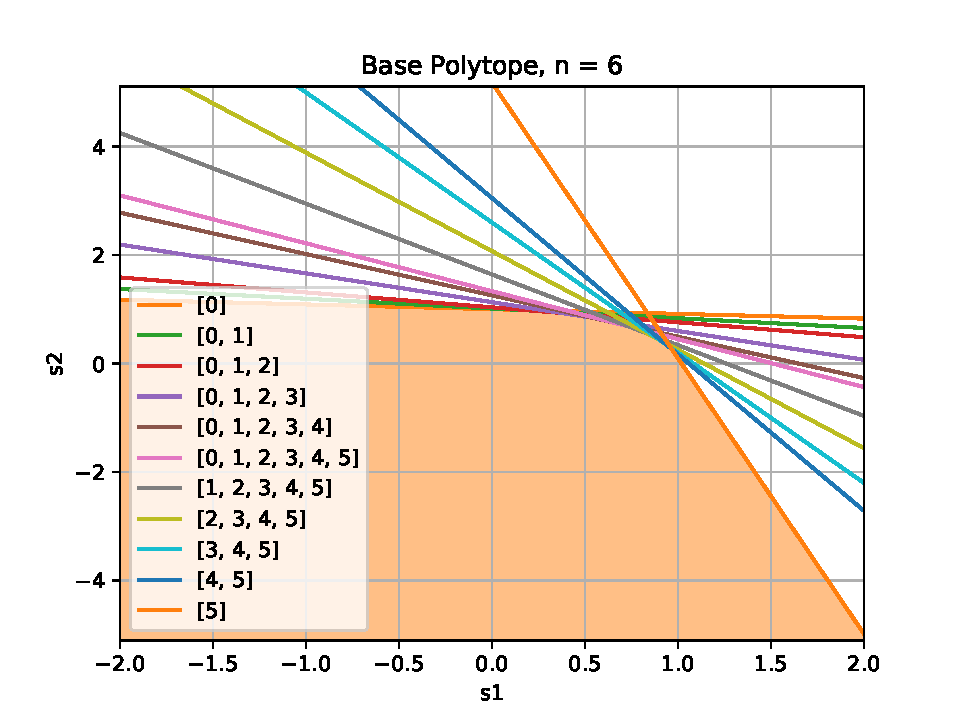
\includegraphics[scale=.75]{base_polytope.pdf}
  \caption{Base polytope for case $n=6$, corresponding to $F(S) = \frac{(\sum_{i \in S}x_i)^2}{\sum_{i \in S}y_i}$, $x = \left\lbrace0.85, 2.05, 2.67, 7.21, 8.2 , 4.03\right\rbrace$, $y = \left\lbrace9.79, 6.35, 4.07, 3.86, 3.45, 0.79\right\rbrace$ }
\end{figure}

\begin{thebibliography}{1}
	\bibitem{PN} Charles A. Pehlivanian, Daniel B. Neill, {\em Efficient Optimization of Partition Scan Statistics via the Consecutive Partitions Property}, preprint, 2021 
	
\end{thebibliography}
\end{document}